\documentclass{ximera}

\input{../preamble.tex}
\author{Elizabeth Campolongo}
\license{Creative Commons Attribution-ShareAlike 4.0 International License}
\acknowledgement{https://spot.pcc.edu/math/orcca/ed2/html/section-technical-definition-of-a-function.html, https://activecalculus.org/prelude/sec-changing-functions-models.html, https://openstax.org/books/college-algebra/pages/3-1-functions-and-function-notation}

\title{Roots}

\begin{document}
\begin{abstract}
  
\end{abstract}
\maketitle

\begin{motivatingQuestions}\begin{itemize}
\item Can we find the inverse of a polynomial?
\item What does it mean to take the $n^{th}$ root of a value?
\end{itemize}\end{motivatingQuestions}


%Recall in Section 3-2-3 that we briefly discussed the square root function..

%Pulling from Elizabeth's lecture notes:

%A {\em root} function is the inverse function of a polynomial of the form $p(x)=x^n$, written $r(x)=\sqrt[n]{x}$. There are two types of root functions: {\em even} roots (where $n$ is even) and {\em odd} roots (where $n$ is odd). In both cases, we have
%
%$$\underbrace{\sqrt[n]{x} \cdot \sqrt[n]{x} \cdot \sqrt[n]{x} \cdot \sqrt[n]{x} \cdots \sqrt[n]{x}}_n =x.$$

Consider the polynomial $p(x) = x^4 + 2x^3 - x^2 - x + 1$. A good question to ask would be whether the function $p$ is invertible. To help us decide, here is the graph of $p(x)$.
\begin{image}
\begin{tikzpicture}
     \begin{axis}[
                domain=-4:4, ymax=15, xmax=5, ymin=-15, xmin=-5, grid = none,
                axis lines =center, xlabel=$x$, ylabel=${y}$,
                ytick={-14,-10,-6,-2,2,6,10,14},
                xtick={-4,-2,2,4},
                ticklabel style={font=\scriptsize},
%                every axis y label/.style={at=(current axis.above origin),anchor=south},
%                every axis x label/.style={at=(current axis.right of origin),anchor=west},
%                axis on top,
                ]
        
        %\addplot [draw=penColor, very thick, smooth, domain=(-7.5:3), <->] {1/(x-3) + 2};
        \addplot [draw=black, thick, smooth, domain=(-2.5:2.5)] {x^4 + 2*x^3 - x^2 - x + 1};2

     %   \addplot [line width=1, gray, dashed,samples=100,domain=(-9:9)] ({3},{x});
        %\addplot [line width=1, gray, dashed,samples=100,domain=(-9:4)] ({x},{2});
    \end{axis}

\end{tikzpicture}
\end{image}

Notice that this graph does not pass the Horizontal Line Test, so the function $p$ is not one-to-one, and therefore not invertible. 

Our polynomial $p(x)$ has many terms, so to simplify the situation, we'll look only at polynomials of the form $x^n$, where $n$ is a positive integer. 

%%%%%%%%%%%%ODD ROOTS
\section{Odd Roots}

Recall that every polynomial $p(x) = x^n$, where $n$ is odd, has the same basic shape. This is demonstrated in the figure below by the graphs of $y = x^n$ for $n = 3, 5,7,9$.

\begin{image}
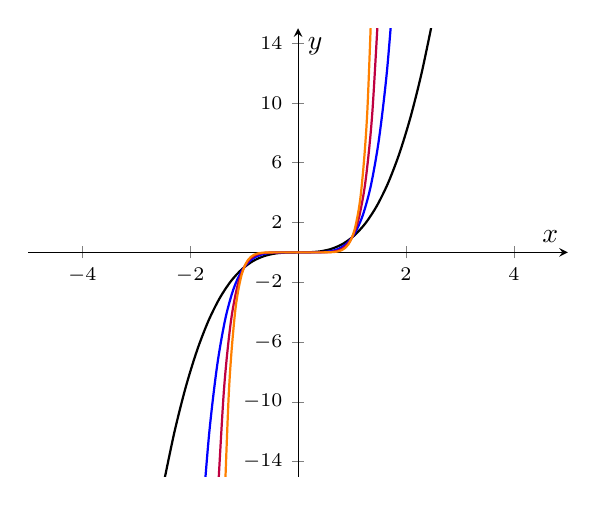
\begin{tikzpicture}
     \begin{axis}[
                domain=-4:4, ymax=15, xmax=5, ymin=-15, xmin=-5, grid = none,
                axis lines =center, xlabel=$x$, ylabel=${y}$,
                ytick={-14,-10,-6,-2,2,6,10,14},
                xtick={-4,-2,2,4},
                ticklabel style={font=\scriptsize},
%                every axis y label/.style={at=(current axis.above origin),anchor=south},
%                every axis x label/.style={at=(current axis.right of origin),anchor=west},
%                axis on top,
                ]
        
        %\addplot [draw=penColor, very thick, smooth, domain=(-7.5:3), <->] {1/(x-3) + 2};
        \addplot [draw=black, thick, smooth, domain=(-2.5:2.5)] {x^3};
         \addplot [draw=blue, thick, smooth, domain=(-1.8:1.8)] {x^5};
          \addplot [draw=purple, thick, smooth, domain=(-1.5:1.5)] {x^7};
           \addplot [draw=orange, thick, smooth, domain=(-1.4:1.4)] {x^9};

     %   \addplot [line width=1, gray, dashed,samples=100,domain=(-9:9)] ({3},{x});
        %\addplot [line width=1, gray, dashed,samples=100,domain=(-9:4)] ({x},{2});
    \end{axis}

\end{tikzpicture}
\end{image}

To see more of how these graphs change with $n$, follow the 
\desmos{viuyei80a0}{800}{600}.



Now, are these functions invertible? Looking at the graphs, we see that these functions pass the Horizontal Line Test. Thus, the functions are one-to-one, and therefore invertible.

\begin{definition}
When $n$ is an odd positive integer, we define \dfn{the $n$th root function} $\sqrt[n]{x}$ to be the inverse of the function defined by $x^n$. The number $n$ is the \dfn{index} of the root, and $x$ is the \dfn{radicand}. We call the symbol $\sqrt{ }$ the \dfn{radical}.
\end{definition}

Let's delve more deeply into the $p(x) = x^3$ example. We have now established that it is invertible, and it's inverse is $r(x)=\sqrt[3]{x}$. 

\begin{exploration}
Draw both functions on the axes provided, then answer the following questions about the function $r(x)$.

\begin{image}
\begin{tikzpicture}
     \begin{axis}[
                domain=-4:4, ymax=9, xmax=9, ymin=-9, xmin=-9,
                axis lines =center, xlabel=$x$, ylabel=${y}$,
               ytick={-8,-6,-4,-2,2,4,6,8},
                xtick={-8,-6,-4,-2,2,4,6,8},
                ticklabel style={font=\scriptsize}
                ]           
           
    \end{axis}

\end{tikzpicture}
\end{image}


\begin{enumerate}
\item What is the $x$-intercept of $r(x)$? 
$(\answer{0} , \answer{0})$

\item What is the $y$-intercept of $r(x)$? 
$(\answer{0} , \answer{0})$

\item What is the domain of $r(x)$? 
$(\answer{-\infty} , \answer{\infty})$

\item What is the range of $r(x)$? 
$(\answer{-\infty} , \answer{\infty})$

\item As $x$ goes to $\infty$, $y$ goes to $\answer{\infty}$.

\item As $x$ goes to $-\infty$, $y$ goes to $\answer{-\infty}$.

\item Does this function have any vertical asymptotes?
\wordChoice{\choice{yes}\choice[correct]{no}}
\end{enumerate}
\end{exploration}

\begin{example}
Below, we have an example of the graph of $y=x^5$ and the two functions

\begin{image}
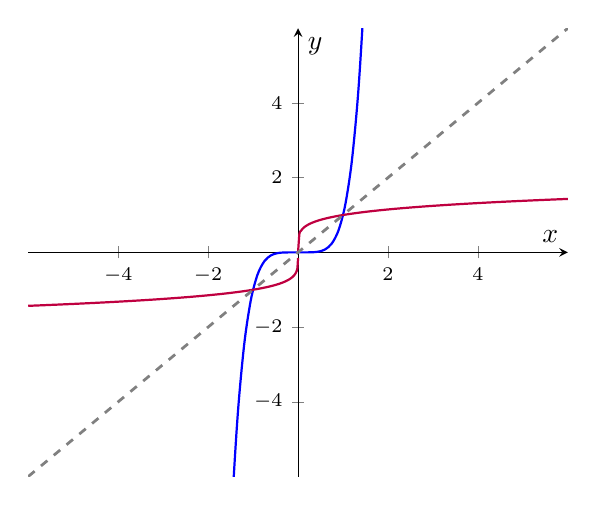
\begin{tikzpicture}
     \begin{axis}[
                domain=-4:4, ymax=6, xmax=6, ymin=-6, xmin=-6,
                axis lines =center, xlabel=$x$, ylabel=${y}$,
               ytick={-4,-2,2,4},
                xtick={-4,-2,2,4},
                ticklabel style={font=\scriptsize}
                ]
        
        %\addplot [draw=penColor, very thick, smooth, domain=(-7.5:3), <->] {1/(x-3) + 2};
       % \addplot [draw=black, thick, smooth, domain=(-2.5:2.5)] {x^3};
         \addplot [draw=blue, thick, smooth, domain=(-1.8:1.8)] {x^5};
          \addplot [draw=purple, samples=200,thick, smooth, domain=(0:6)] {x^(1/5)};
            \addplot [draw=purple, samples=400, thick, smooth, domain=(-6:0)] {-(-x)^(1/5)};
        %   \addplot [draw=orange, thick, smooth, domain=(-1.4:1.4)] {x^9};

       \addplot [line width=1, gray, dashed,samples=100,domain=(-6:6)] {x};
        %\addplot [line width=1, gray, dashed,samples=100,domain=(-9:4)] ({x},{2});
    \end{axis}

\end{tikzpicture}
\end{image}

\end{example}

Recall that a function $f$ is {\em even} if $f(-x) = f(x)$ for all $x$ in its domain, and $f$ is {\em odd} if $f(-x) = -f(x)$ for all $x$. Otherwise, the function is neither. % Recall that these properties are reflected in the graph of the function. An even function is reflected across a single axis, while an odd function is reflected across both.
Let's consider an example. Given $x=8$, $r(x) = \sqrt[3]{8}=2$ and $r(-x) = \sqrt[3]{-8} = -2$, since $(-2)\cdot(-2)\cdot(-2) =(4)\cdot(-2) = -8$. Based on this example, do you think $r(x)$ is even, odd, or neither?

If you guessed odd, then you are correct! All odd-index root functions are odd functions. 
%We can show this through the associativity and commutativity of multiplication. 
%Consider $r(x) = \sqrt[n]{x} = y$ for $n$ odd, then we know that $\underbrace{y \cdot y \cdot y \cdots y}_n=x$, so
%\begin{align*}
%\underbrace{(-y) \cdot (-y) \cdot (-y) \cdots (-y)}_n 
%&= \underbrace{(-1) \cdot (-1) \cdot (-1) \cdots (-1)}_n \cdot \underbrace{y \cdot y \cdot y \cdots y}_n \\
%&= (-1) \cdot x = -x.
%\end{align*}
%Thus, $r(-x) = \sqrt[n]{-x} = -y = -\sqrt[n]{x} = -r(x)$, meaning $r$ is an odd function.
%It is important to note that the parentheses around the ``-1" terms are {\bf not} optional. 



%%%%%%%%%%%%EVEN ROOTS
\section{Even Roots}
We again begin by recalling the general shape of $p(x) = x^n$, but this time for $n$ {\em even}. These functions also have the same basic shape for all even $n$. This is demonstrated by the graphs of $y = x^n$ for $n = 2,4,6,8$ given below.

\begin{image}
\begin{tikzpicture}
     \begin{axis}[
                domain=-4:4, ymax=7, xmax=5, ymin=-2, xmin=-5,
                axis lines =center, xlabel=$x$, ylabel=${y}$,
                ytick={-1,1,2,3,4,5,6},
                xtick={-4,-3,-2,-1,1,2,3,4},
                ticklabel style={font=\scriptsize},
%                every axis y label/.style={at=(current axis.above origin),anchor=south},
%                every axis x label/.style={at=(current axis.right of origin),anchor=west},
%                axis on top,
                ]
        
        %\addplot [draw=penColor, very thick, smooth, domain=(-7.5:3), <->] {1/(x-3) + 2};
        \addplot [draw=black, thick, smooth, domain=(-2.8:2.8)] {x^2};
         \addplot [draw=blue, thick, smooth, domain=(-1.8:1.8)] {x^4};
          \addplot [draw=purple, thick, smooth, domain=(-1.5:1.5)] {x^6};
           \addplot [draw=orange, thick, smooth, domain=(-1.4:1.4)] {x^8};
           
           
         %  \node[label = right:{$y=x^2$}] at (5,4) {};

     %   \addplot [line width=1, gray, dashed,samples=100,domain=(-9:9)] ({3},{x});
        %\addplot [line width=1, gray, dashed,samples=100,domain=(-9:4)] ({x},{2});
        
          %\addplot[color=penColor,fill=penColor,only marks,mark=*] coordinates{(-6,5)};
        %\addplot[color=penColor,fill=white,only marks,mark=*] coordinates{(-6,1.88)};
        \addplot[label = right:{$y=x^2$}] coordinates{(2,5)};
        \addplot[color=penColor,fill=white,only marks,mark=*] coordinates{(6,-2)};
    \end{axis}

\end{tikzpicture}
\end{image}

To see more of how these graphs change with $n$, follow the
\desmos{qpqwtrppqt}{800}{600}.

Now, are these functions invertible? All of the graphs in the figure above are symmetric about the $y$-axis (example $2^2 = 4 = (-2)^2$), so they do {\em not} pass the horizontal line test. Thus, these functions are {\em not} one-to-one, and therefore {\em not} invertible.

So, how can we define an even root function? For example, what does $\sqrt{x}$ really mean, and how is it related to $x^2$?

Consider the polynomial $p(x)=x^2$, graphed below with its inverse relation $\{(x^2, x): x \text{ is a real number}\}$.
% to the polynomial $p(x) = x^2$. Observing the graph below, we see that by restricting the domain of $p$ to $x \geq 0$, we now have a function which passes the horizontal line test, and can thus be inverted.
\begin{image}
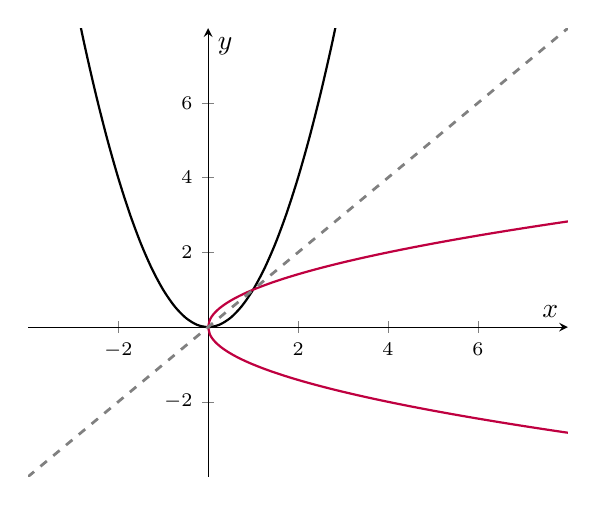
\begin{tikzpicture}
     \begin{axis}[
                domain=-4:4, ymax=8, xmax=8, ymin=-4, xmin=-4,
                axis lines =center, xlabel=$x$, ylabel=${y}$,
               ytick={-2,2,4, 6},
                xtick={-2,2,4,6},
                ticklabel style={font=\scriptsize}
                ]
        
        %\addplot [draw=penColor, very thick, smooth, domain=(-7.5:3), <->] {1/(x-3) + 2};
       % \addplot [draw=black, thick, smooth, domain=(-2.5:2.5)] {x^3};
         \addplot [draw=black, thick, smooth, domain=(-3:3)] {x^2};
          \addplot [draw=purple, samples=200,thick, smooth, domain=(0:8)] {x^(1/2)};
            \addplot [draw=purple, samples=200, thick, smooth, domain=(0:8)] {-x^(1/2)};
        %   \addplot [draw=orange, thick, smooth, domain=(-1.4:1.4)] {x^9};

       \addplot [line width=1, gray, dashed,samples=100,domain=(-6:8)] {x};
        %\addplot [line width=1, gray, dashed,samples=100,domain=(-9:4)] ({x},{2});
    \end{axis}

\end{tikzpicture}
\end{image}

Observe that by restricting the domain of $p$ to $x \geq 0$, we now have a function which passes the horizontal line test, and can thus be inverted. The following picture illustrates the situation.

\begin{image}
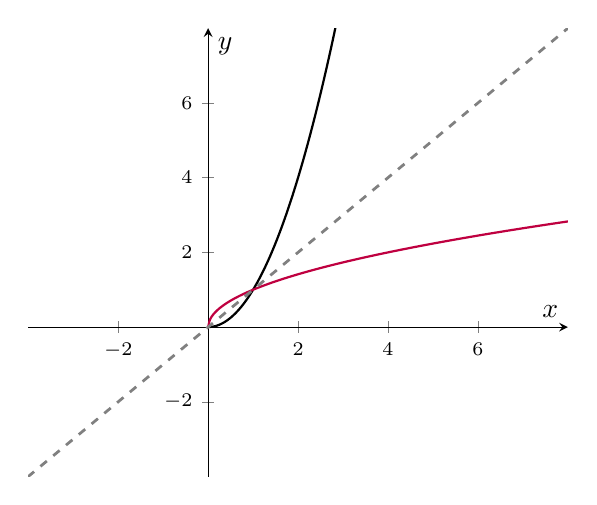
\begin{tikzpicture}
     \begin{axis}[
                domain=-4:4, ymax=8, xmax=8, ymin=-4, xmin=-4,
                axis lines =center, xlabel=$x$, ylabel=${y}$,
               ytick={-2,2,4, 6},
                xtick={-2,2,4,6},
                ticklabel style={font=\scriptsize}
                ]
        
        %\addplot [draw=penColor, very thick, smooth, domain=(-7.5:3), <->] {1/(x-3) + 2};
       % \addplot [draw=black, thick, smooth, domain=(-2.5:2.5)] {x^3};
         \addplot [draw=black, thick, smooth, domain=(0:3)] {x^2};
          \addplot [draw=purple, samples=200,thick, smooth, domain=(0:8)] {x^(1/2)};
          %  \addplot [draw=purple, samples=200, thick, smooth, domain=(0:8)] {-x^(1/2)};
        %   \addplot [draw=orange, thick, smooth, domain=(-1.4:1.4)] {x^9};

       \addplot [line width=1, gray, dashed,samples=100,domain=(-6:8)] {x};
        %\addplot [line width=1, gray, dashed,samples=100,domain=(-9:4)] ({x},{2});
    \end{axis}

\end{tikzpicture}
\end{image}

%
%\begin{image}
%\begin{tikzpicture}
%     \begin{axis}[
%                domain=-4:4, ymax=7, xmax=5, ymin=-2, xmin=-5,
%                axis lines =center, xlabel=$x$, ylabel=${y}$,
%                ytick={-1,1,2,3,4,5,6},
%                xtick={-4,-3,-2,-1,1,2,3,4},
%                ticklabel style={font=\scriptsize},
%%                every axis y label/.style={at=(current axis.above origin),anchor=south},
%%                every axis x label/.style={at=(current axis.right of origin),anchor=west},
%%                axis on top,
%                ]
%        
%        %\addplot [draw=penColor, very thick, smooth, domain=(-7.5:3), <->] {1/(x-3) + 2};
%        \addplot [draw=black, thick, smooth, domain=(-2.8:2.8)] {x^2};
%%         \addplot [draw=blue, thick, smooth, domain=(-1.8:1.8)] {x^4};
%%          \addplot [draw=purple, thick, smooth, domain=(-1.5:1.5)] {x^6};
%%           \addplot [draw=orange, thick, smooth, domain=(-1.4:1.4)] {x^8};
%           
%           
%         %  \node[label = right:{$y=x^2$}] at (5,4) {};
%
%     %   \addplot [line width=1, gray, dashed,samples=100,domain=(-9:9)] ({3},{x});
%        %\addplot [line width=1, gray, dashed,samples=100,domain=(-9:4)] ({x},{2});
%        
%          %\addplot[color=penColor,fill=penColor,only marks,mark=*] coordinates{(-6,5)};
%        %\addplot[color=penColor,fill=white,only marks,mark=*] coordinates{(-6,1.88)};
%        \addplot[label = right:{$y=x^2$}] coordinates{(2,5)};
%        \addplot[color=penColor,fill=white,only marks,mark=*] coordinates{(6,-2)};
%    \end{axis}
%
%\end{tikzpicture}
%\end{image}

% The relation to find this inverse is $x=y^2$, but the function will be $y = \sqrt{x}$. 
Now, our inverse relation is actually a function, since it passes the Horizontal Line Test. Therefore, if we let $p(x) = x^2$ for $x \geq 0$, we can then define $r(x) = \sqrt[2]{x} = \sqrt{x}$ as the inverse function of $p(x)$ on this restricted domain.

\begin{definition}
When $n$ is an even positive integer, we define \dfn{the $n$th root function} $\sqrt[n]{x}$ to be the inverse of the function defined by $x^n$ restricted to the domain $x \ge 0$.
\end{definition}

\begin{exploration}
We now repeat Exploration 1 for $r(x) = \sqrt[4]{x}$. Draw both functions on the axes provided, then answer the following questions about the function $r(x)$.

\begin{image}
\begin{tikzpicture}
     \begin{axis}[
                 domain=-4:4, ymax=7, xmax=5, ymin=-2, xmin=-5,
                axis lines =center, xlabel=$x$, ylabel=${y}$,
                ytick={-1,1,2,3,4,5,6},
                xtick={-4,-3,-2,-1,1,2,3,4},
                ticklabel style={font=\scriptsize},
                ]           
           
    \end{axis}

\end{tikzpicture}
\end{image}

\begin{enumerate}
\item What is the $x$-intercept of $r(x)$? 
$(\answer{0} , \answer{0})$

\item What is the $y$-intercept of $r(x)$? 
$(\answer{0} , \answer{0})$

\item What is the domain of $r(x)$? 
$[\answer{0} , \answer{\infty})$

\item What is the range of $r(x)$? 
$[\answer{0} , \answer{\infty})$

\item As $x$ goes to $\infty$, $y$ goes to $\answer{\infty}$.

\item Does this function have any vertical asymptotes?
\wordChoice{\choice{yes}\choice[correct]{no}}
\end{enumerate}
\end{exploration}

One question we might ask is whether $r(x) = \sqrt{x}$ and $p(x) = x^2$ are truly inverses. The answer may seem like an obvious ``yes!'', but since we restricted the domain of $p$ in order to define $r$, we need to check. To check whether $r$ and $p$ are inverses, we need to confirm that $r(p(x)) = \sqrt{x^2} = x$ and $p(r(x)) = (\sqrt{x})^2 = x$. That is, when we plug in a number to $\sqrt{x^2}$ and $(\sqrt{x})^2$, we should get the same number as the output. Let's try plugging in $-1$ to $r(p(x))$. This gives us 
$$
r(p(-1)) = r((-1)^2) = \sqrt{(-1)^2} = \sqrt{1} = 1,
$$
which is not the same as $-1$. If we repeat this process with a few more numbers, we find that $\sqrt{(-2)^2} = 2$, $\sqrt{1^2} = 1$, $\sqrt{(-45)^2} = 45$, and $\sqrt{98^2} = 98$. We can conclude that $\sqrt{x^2}$ is a function that takes its input and returns its absolute value. That is, $\sqrt{x^2} = |x|$. Since $\sqrt{x^2} = r(p(x))$, we conclude that $r(p(x))$ does not output its input, and therefore, $r$ and $p$ are not inverses. This is something that will be extremely important when solving equations using even roots. 

Now, what if we instead restricted our domain to $x \leq 0$? Consider $q(x) = x^2$ defined for $x \leq 0$. The graph of this function is below.

\begin{image}
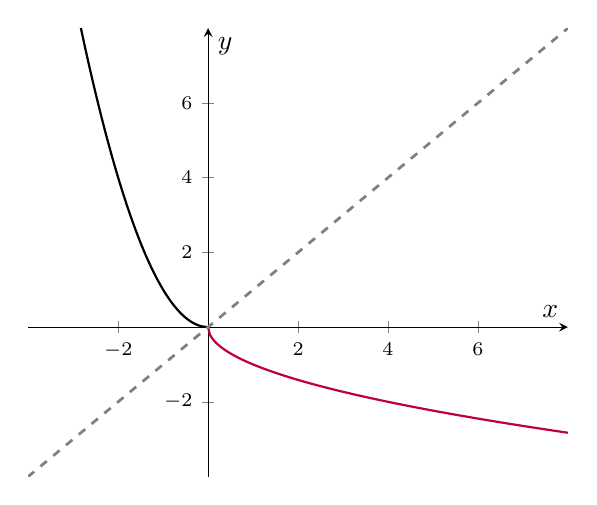
\begin{tikzpicture}
     \begin{axis}[
                domain=-4:4, ymax=8, xmax=8, ymin=-4, xmin=-4,
                axis lines =center, xlabel=$x$, ylabel=${y}$,
               ytick={-2,2,4, 6},
                xtick={-2,2,4,6},
                ticklabel style={font=\scriptsize}
                ]
        
        %\addplot [draw=penColor, very thick, smooth, domain=(-7.5:3), <->] {1/(x-3) + 2};
       % \addplot [draw=black, thick, smooth, domain=(-2.5:2.5)] {x^3};
         \addplot [draw=black, thick, smooth, domain=(-3:0)] {x^2};
         % \addplot [draw=purple, samples=200,thick, smooth, domain=(0:8)] {x^(1/2)};
           \addplot [draw=purple, samples=200, thick, smooth, domain=(0:8)] {-x^(1/2)};
        %   \addplot [draw=orange, thick, smooth, domain=(-1.4:1.4)] {x^9};

       \addplot [line width=1, gray, dashed,samples=100,domain=(-6:8)] {x};
        %\addplot [line width=1, gray, dashed,samples=100,domain=(-9:4)] ({x},{2});
    \end{axis}

\end{tikzpicture}
\end{image}
By the Horizontal Line Test, this restriction is one-to-one, and therefore invertible. The inverse of this function as shown above is $s(x) = -\sqrt{x} = -r(x)$.

%Hence, if we wish to find all values that undo $y=x^2$, then we must consider both $y = \sqrt{x}$ and $y=-\sqrt{x}$. It is important to note that this is true for {\em all} even roots. 
%We can show this in the same way that we showed odd root functions are odd functions. 
%Consider $r(x) = \sqrt[n]{x} = y$ for $n$ even, then we know that $\underbrace{y \cdot y \cdot y \cdots y}_n=x$, so
%\begin{align*}
%\underbrace{(-y) \cdot (-y) \cdot (-y) \cdots (-y)}_n 
%&= \underbrace{(-1) \cdot (-1) \cdot (-1) \cdots (-1)}_n \cdot \underbrace{y \cdot y \cdot y \cdots y}_n \\
%&= (1) \cdot x = x.,
%\end{align*}
%since we have $(-1)^2 = 1$ multiplied $\frac{n}{2}$ times.

%
%%This exemplifies the fact that, 
%In general, the square root is not one-to-one when used for {\em solving} equations. Instead, the output must be chosen. For instance, the square root of 9 is 3, since the square root {\em function} is only defined on $[0,\infty)$. However, if we wish to solve the equation $x^2=9$, the solution is not $x=3$, or, to be more precise, there are \textbf{two} solutions: $x=3$ \textbf{and} $x = -3$, since both $3^2$ and $(-3)^2$ are equal to 9. This can be demonstrated by solving the equation through factoring:
%$$0=x^2-9 =(x+3)(x-3),$$
%which has {\em two} solutions: $x=3$ and $x = -3$.
%
%$\sqrt{}$ is not one-to-one so you must {\em choose} which value makes sense in the context, or list both.

%We now formalize the definition of the $n^{th}$ root function for a general positive integer $n$.
%
%\begin{definition}
%For any real number $x$, the $n^{th}$ root of $x$ is denoted by 
%$$\sqrt[n]{x} = x^{\frac{1}{n}}.$$
%%
%It is further defined as the real number $y$ such that 
%$$y^n = x.$$
%Note that if $n$ is \textbf{even}, then both $y^n$ and $(-y)^n$ will be equal to $x$, so for this to be a {\em function}, we must choose one or the other. The {\em principal} $n^{th}$ root is the positive value, $|y|$. %since we define the $n^{th}$ root {\em function} to produce values in $[0,\infty)$ for $n$ even as with the more-common square root. 
%Further note that the input of an even $n^{th}$ root (the $x$ in $\sqrt[n]{x}$) must be in $[0,\infty)$. % as well.
%
%However, if $n$ is \textbf{odd}, then there is only one such $y$, and {\em both} the input and output of the $n^{th}$ root function are in $(-\infty,\infty)$.
%\end{definition}

\begin{example}
We demonstrate a few common even and odd $n^{th}$ roots to highlight this distinction.
\begin{enumerate}
\item $\sqrt[3]{8} = 2$, since $2 \cdot 2 \cdot 2 = 8$.

\item $\sqrt[3]{-8} = - 2$, since $-2 \cdot (-2) \cdot (-2) = 4 \cdot (-2) = -8$.

\item $\sqrt[4]{16} = 2$, since $2 \cdot 2 \cdot 2 \cdot 2 \cdot 2 = 4 \cdot 4 = 16$. However, the $4^{th}$ root of -16 is not defined.

\item $\sqrt[4]{0} =0$, since zero times any number is always zero. This is {\em the} example of an even $n^{th}$ root that has only {\em one} solution.

\item Likewise, $\sqrt[125]{0} = 0$.
\end{enumerate}
\end{example}

\section{Using Roots to Solve Equations}
If we are asked to find all values $x$ such that $x^2=4$, then the question is asking which values of $x$ multiplied by themselves give 4. In other words, find $x$ such that $x \cdot x$ is equal to 4. It is simple to see that there are two values which make this true:
%$$x\cdot x = 1\cdot x \cdot x = (-1)^2 \cdot x \cdot x = -1 \cdot x \cdot (-1)\cdot x = -x \cdot (-x),$$
$$2\cdot 2 = 4 \text{ and } (-2) \cdot (-2) = 4.$$
%by the distributive property of multiplication. Thus, both $x$ and $-x$ will be solutions. 
In solving an equation, it is common to express this as follows.
\begin{align*}
x^2 &= 4 \\
\sqrt{x^2} &= \sqrt{4} \\
|x| &= 2 \\
x &= \pm 2.
\end{align*}
%This is because the square root of a number is always non-negative; {\em however}, we are looking for the value that makes this equation true, and s
Since $f(x)=x^2$ is \textbf{not} one-to-one, there are two values of $x$ which make it equal to any positive number, as demonstrated in the following graph.

\begin{image}
\begin{tikzpicture}
     \begin{axis}[
                domain=-8:8, ymax=8, xmax=8, ymin=-8, xmin=-8,
                axis lines =center, xlabel=$x$, ylabel=${y}$,
               ytick={-6,-4,-2,2,4, 6},
                xtick={-6,-4,-2,2,4,6},
                ticklabel style={font=\scriptsize}
                ]
        
        %\addplot [draw=penColor, very thick, smooth, domain=(-7.5:3), <->] {1/(x-3) + 2};
       % \addplot [draw=black, thick, smooth, domain=(-2.5:2.5)] {x^3};
         \addplot [draw=black, thick, smooth, domain=(-3:3)] {x^2};
	\addplot [draw=penColor2, thick, smooth, domain=(-8:8)] {4};
          %\addplot [draw=purple, samples=200,thick, smooth, domain=(0:8)] {x^(1/2)};
            %\addplot [draw=purple, samples=200, thick, smooth, domain=(0:8)] {-x^(1/2)};
        %   \addplot [draw=orange, thick, smooth, domain=(-1.4:1.4)] {x^9};

       %\addplot [line width=1, gray, dashed,samples=100,domain=(-6:8)] {x};
        %\addplot [line width=1, gray, dashed,samples=100,domain=(-9:4)] ({x},{2});
    \end{axis}

\end{tikzpicture}
\end{image}

%do \textbf{not} restrict the range of the $n^{th}$ root to $[0,\infty)$, but allow it to produce a negative value. In this case, the $n^{th}$ root is no longer one-to-one for even $n$.

\begin{example}
\begin{enumerate}
\item Solve the equation $x^3 = 8$. 

Taking the cube root on both sides, we find that 
\begin{align*}
\sqrt[3]{x^3} &= \sqrt[3]{8} \\
x &= 2.
\end{align*}

Note that $\sqrt[3]{x^3} = x$, since 3 is odd, and odd roots are really inverses to their corresponding power functions. 

\item Solve the equation $x^3 = -8$. 

Taking the cube root on both sides, we find that 
\begin{align*}
\sqrt[3]{x^3} &= \sqrt[3]{-8} \\
x &= -2.
\end{align*}

\item Solve the equation $x^2 = 16$. 

Taking the square root on both sides, we find that 
\begin{align*}
\sqrt{x^2} &= \sqrt{16} \\
|x| &= 4\\
x &= \pm 4.
\end{align*}
Therefore, there are two solutions to this equation: $-4$ and $4$.

\item Solve the equation $2x^4 - 4= 28$. 

First, rearrange the equation. Add 4 to both sides to find $2x^4 = 32$. Divide both sides by 2 to find $x^4 = 16$. Taking the 4th root on both sides, we find that 
\begin{align*}
\sqrt[4]{x^4} &= \sqrt[4]{16} \\
|x| &= 2\\
x &= \pm 2.
\end{align*}
Therefore, there are two solutions to this equation: $-2$ and $2$.

Recall that for any even integer $n$, $\sqrt[n]{x^n} = |x|$. 

\item Solve the equation $-3x^4= 32$. 

First, rearrange the equation by dividing both sides by -3. This yields $x^4 = -\frac{32}{3}$. Taking the 4th root on both sides, we find that 
\begin{align*}
\sqrt[4]{x^4} &= \sqrt[4]{-\frac{32}{3}} \\
|x| &= \sqrt[4]{-\frac{32}{3}}.
\end{align*}
Since any even-index root of a negative number is not defined, there are no solutions to this equation.

\end{enumerate}
\end{example}

These examples illustrate a general principle that is good to have in your toolbox for solving equations. If $a^3=b$, then we know that $a = \sqrt[3]{b}$. This is true for any odd powers. However, if $a^2 =b$, then {\bf either} $a=\sqrt{b}$ {\bf or} $a = -\sqrt{b}$. This is true for any even powers.  

\section{Finding $x$-intercepts of a Quadratic in Vertex Form}

Now, we can use our understanding of the squareroot function to find the $x$-intercepts of a quadratic given in vertex form.

\begin{example}
Find the $x$-intercepts of the quadratic $2(x-3)^2-5= 0$ which is written in vertex form. 

\begin{explanation}
First, rearrange the equation by adding $5$ to both sides. This yields $$2(x-3)^2 = 5.$$ Then divide each side by $2$, resulting in $$(x-3)^2 = \frac{5}{2}.$$ Taking the square root on both sides, we find that 
\begin{align*}
\sqrt{(x-3)^2} &= \sqrt{\frac{5}{2}} \\
|x-3| &= \sqrt{\frac{5}{2}}\\
x-3 &= \pm \sqrt{\frac{5}{2}}\\
x &= 3 \pm \sqrt{\frac{5}{2}}
\end{align*}
\end{explanation}
\end{example}

Notice that this gives us a third method for finding the roots ($x$-intercepts) of a quadratic in general. We can use any of these methods to solve a quadratic.
\begin{enumerate}
\item Factor the quadratic and write it in Root Form
\item Use the quadratic formula to find the roots
\item Write the quadratic in vertex form and then solve using a squareroot
\end{enumerate}

Mathematically, these last two methods are actually related.  The quadratic formula is just what happens when you rewrite the general quadratic $f(x)=ax^2+bx+c$ in vertex form and then solve for $x$!


%\begin{callout}
%{\bf Important Algebra Note:}\\
%If $a^3=b$, then we know that $a = \sqrt[3]{b}$.
%
%However, if $a^2 =b$, then {\bf either} $a=\sqrt{b}$ {\bf or} $a = -\sqrt{b}$.
%\\
%
%{\bf In General:}\\
%For $n$ {\bf odd}, 
%$$\text{ if } a^n = b, \text{ then } a=\sqrt[n]{b}.$$
%
%For $n$ {\bf even},
%$$\text{ if } a^n = b, \text{ then {\bf either} } a=\sqrt[n]{b} \textbf{ or } a = -\sqrt{b}.$$
%
%\end{callout}

%\begin{callout}
%{\bf Warning:} Solving an equation like $x^2 = 4$ is very different than computing $\sqrt{4} = 2$. To solve the equation, one rewrites it as $x^2-4=0$, then factors it as $(x-2)(x+2) = 0$, and concludes that $x=-2$ or $x=2$. However, people often write this sloppily as $x = \pm 2$, and proceed to say {\bf wrong} things such as $\sqrt{4} = \pm 2$. Square roots are always non-negative, so $\sqrt{4}=2$ is the only correct equality. To relate this back with solving the equation $x^2=4$, one could alternatively take the square root of both sides, leading to $\sqrt{x^2} = \sqrt{4}$. The square root of a square is not the original number, but its absolute value instead. This means that instead of writing the next step as $x=2$ (which would lead us to miss the solution $x=-2$), we should write $|x| = 2$. Which real numbers have absolute value equal to $2$? Just $x=2$ and $x=-2$.
%
%This is true for any {\em even} root, for instance, consider the equation $x^4 = 16$. If we take the fourth root ($\sqrt[4]{}$) of both sides, we then have $x = \pm 2$. However, if we have $x^3 = 8$, when we take the third root, we get only one solution, $x=2$. Factoring, we can see why this is the case: $x^3=8$ is equivalent to 
%$$0=x^3 - 8=(x-2)(x^2+2x+4),$$
%which has only one real solution, $x=2$.
%
%However, {\em odd} roots have the unique property that they can be applied to {\em negative} numbers. Following the pattern above, $x^2=-4$ has no real solutions since the square root is only defined for values greater or equal to zero. However, $x^3=-8$ does have a solution: $x=-2$, we can check this easily by multiplying out 
%$$(-2)^3=(-2)\cdot(-2)\cdot(-2) = 4 \cdot (-2) = -8.$$
%It is important to note that the parentheses around the ``-2" terms are {\bf not} optional. 
%\end{callout}

\begin{summary}
In general, we are not able to simply find the inverse of polynomials.

However, when the polynomial is $p(x) = x^n$ for a positive {\em odd} integer $n$, the polynomial is invertible as the $n^{th}$ root function $r(x) = \sqrt[n]{x}$.

When $n$ is {\em even}, it is possible to define an inverse function $r(x) = \sqrt[n]{x}$ on a restricted domain of $[0, \infty)$. The $n^{th}$ root is defined as the inverse of $p(x)$ on the restricted domain $[0,\infty)$.
\end{summary}



\end{document}